% =====================================================================================
% Odbrana projekta iz Računarskog vida -- prezentacija
%
% Gradi se sa pdflatex (dva prolaza zbog \totalframenumber):
%     pdflatex prezentacija.tex && pdflatex prezentacija.tex
%
% BEZ babel paketa, iz istog razloga kao i izveštaj. Babel-ov `serbian` po
% podrazumevanim podešavanjima daje ĆIRILICU i zahteva serbian.ldf, koji na ovoj mašini
% nije instaliran. utf8 + T1 + Fira renderuju srpsku latinicu ispravno, što je provereno
% na š đ č ć ž i Š Đ Č Ć Ž.
%
% Slike se čitaju iz figures/report/, iste one koje su u izveštaju. One su namerno bez
% ugrađenog naslova, pa se na slajdu naslov daje okvirom, a u izveštaju natpisom ispod.
% =====================================================================================
\documentclass[aspectratio=169, 10pt]{beamer}

\usetheme{metropolis}
\usepackage[utf8]{inputenc}
\usepackage[T1]{fontenc}
\usepackage[sfdefault]{FiraSans}
\usepackage{FiraMono}
\usepackage{graphicx}
\usepackage{booktabs}
\usepackage{appendixnumberbeamer}   % dodatni slajdovi se ne broje u ukupan broj
\usepackage{tikz}
\usetikzlibrary{positioning, arrows.meta}

\graphicspath{{../../figures/report/}}

\metroset{block=fill, numbering=fraction, progressbar=frametitle}

\definecolor{Naglasak}{HTML}{C05621}
\setbeamercolor{alerted text}{fg=Naglasak}

% Uže margine za tabele koje su široke
\newcommand{\uska}{\setlength{\tabcolsep}{4pt}\small}

% --- Stilovi za dijagrame crtane u TikZ-u ---------------------------------------------
% Dijagrami se crtaju ovde umesto u PlantUML-u, jer je slajd 16:9, a PlantUML raspored za
% ovakav lanac daje odnos stranica od preko 6:1, na kome bi tekst pao ispod čitljivog.
\tikzset{
  modul/.style   = {rectangle, rounded corners=2pt, draw=gray!60, fill=gray!8,
                    text=gray!55, align=center, font=\scriptsize,
                    minimum height=1.05cm, text width=2.05cm},
  modulmvp/.style= {rectangle, rounded corners=2pt, draw=Naglasak, very thick,
                    fill=Naglasak!12, text=black, align=center, font=\scriptsize,
                    minimum height=1.05cm, text width=2.05cm},
  kutija/.style  = {rectangle, rounded corners=2pt, draw=gray!55, align=center,
                    font=\scriptsize, minimum height=0.72cm, inner sep=3pt},
  ulaz/.style    = {kutija, fill=yellow!12},
  trening/.style = {kutija, fill=green!10},
  test/.style    = {kutija, fill=blue!8},
  degr/.style    = {kutija, fill=red!8, draw=Naglasak},
  tok/.style     = {-{Stealth[length=4pt]}, draw=gray!70},
  tokis/.style   = {-{Stealth[length=4pt]}, draw=gray!70, dashed},
}

\title{Uporedna analiza reprezentacija slike primenjenih na klasifikaciju saobraćajnih znakova pri kontrolisanim degradacijama ulaza}
\author{Mihajlo Madić, 2119}
\institute{Univerzitet u Nišu, Elektronski fakultet \\ Projekat iz predmeta Računarski vid}
\date{Niš, 2026.}

\begin{document}

\maketitle

% =====================================================================================
\section{Motivacija i postavka}

\begin{frame}{Kontekst projekta u širem sistemu}

Kompletan sistem za razumevanje saobraćajne signalizacije iz video snimka može biti razložen na
\alert{pet modula}.

\vspace{0.35cm}
\begin{center}
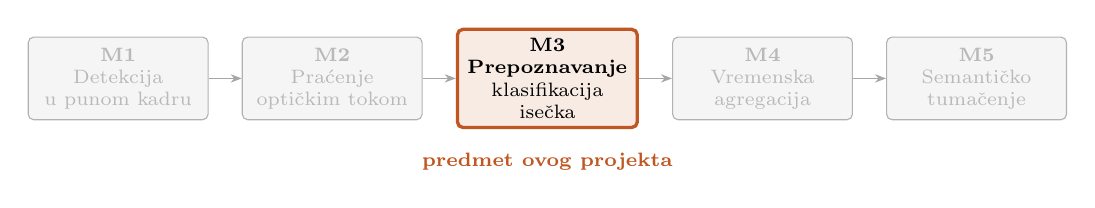
\begin{tikzpicture}[node distance=0.42cm]
  \node[modul]                      (m1) {\textbf{M1}\\Detekcija\\u punom kadru};
  \node[modul,    right=of m1]      (m2) {\textbf{M2}\\Praćenje\\optičkim tokom};
  \node[modulmvp, right=of m2]      (m3) {\textbf{M3}\\\textbf{Prepoznavanje}\\klasifikacija isečka};
  \node[modul,    right=of m3]      (m4) {\textbf{M4}\\Vremenska\\agregacija};
  \node[modul,    right=of m4]      (m5) {\textbf{M5}\\Semantičko\\tumačenje};

  \draw[tok] (m1) -- (m2);
  \draw[tok] (m2) -- (m3);
  \draw[tok] (m3) -- (m4);
  \draw[tok] (m4) -- (m5);

  \node[below=0.18cm of m3, font=\scriptsize\bfseries, text=Naglasak]
        (oznaka) {predmet ovog projekta};
\end{tikzpicture}
\end{center}

\vspace{0.15cm}
\small
Ovaj projekat realizuje \alert{isključivo modul M3}, i to nad isečcima čije granice daje
anotacija skupa podataka, umesto izlaza detektora. Ostali moduli se opisuju radi
kontekstualizacije, jer se ne implementiraju i ne evaluiraju.

\end{frame}

\begin{frame}{Zašto još jedan rad o GTSRB skupu}

GTSRB je \alert{zasićen benchmark}. Savremene konvolucione mreže prelaze $99\%$ tačnosti,
pa još jedan broj u toj koloni ne donosi ništa novo.

\begin{block}{Pitanje koje ovaj rad postavlja}
Umesto ,,koja reprezentacija je najbolja'', pita se \alert{koja reprezentacija se kako ponaša pod
kojim uslovima}.
\end{block}

Onaj koji bira reprezentaciju slike ne bira za laboratorijske, već realne uslove - noć, kiša, zamućenje usled kretanja...
Rang-lista po odabranoj metrici, na čistim podacima, za tu odluku možda nije dovoljna.

\end{frame}

\begin{frame}{Četiri reprezentacije, četiri različite strukture}

Metode se razlikuju po nekoliko strukturnih osa istovremeno, pa se očekuje da će i otkazivati
na različite načine.

\begin{center}
\uska
\begin{tabular}{lccc}
\toprule
\textbf{Reprezentacija} & \textbf{Prostorna struktura} & \textbf{Lokalnost} & \textbf{Uči se?} \\
\midrule
PCA  & holistička, osetljiva na poravnanje & globalna & ne \\
HOG  & kruta mreža, raspored očuvan        & lokalna  & ne \\
BoVW & \alert{bez prostornog rasporeda}    & lokalna  & samo rečnik \\
CNN  & hijerarhijska, otporna na pomeraj   & lokalna  & u potpunosti \\
\bottomrule
\end{tabular}
\end{center}

\vspace{0.3cm}
Konvoluciona mreža se pojavljuje \alert{dvaput}, kao ekstraktor obeležja ispred istog
linearnog SVM-a i kao mreža sa sopstvenom softmax glavom. Time se dobija \alert{pet
konfiguracija}.

\end{frame}

\begin{frame}{Šta je fiksirano, i kako se sprovodi eksperiment}

Da bi razlika u rezultatu bila pripisiva \alert{isključivo reprezentaciji}, sve ostalo mora
biti identično.

\begin{itemize}
  \item \textbf{Klasifikator} je \texttt{LinearSVC} za sve metode, uz isti protokol izbora.
  \item \textbf{Pretprocesiranje} je fiksirano na \texttt{raw\_gray} za celo poređenje.
  \item \textbf{Podela} na trening i validaciju je po sekvencama, nikako po slikama.
  \item \textbf{Evaluacija} koristi makro-F1 kao glavnu meru, zbog neuravnoteženosti
        od $10{,}7\times$.
  \item \textbf{Test skup} je dodirnut tačno jednom, pri finalnoj evaluaciji.
\end{itemize}

\begin{alertblock}{Posledica}
Sve što mora biti isto za svih pet metoda živi u biblioteci \texttt{gtsrb}, koju skripte samo
pozivaju, pa se sve evaluacije izvršavaju nad jedinstvenim protokolom.
\end{alertblock}

\end{frame}

% =====================================================================================
\section{Metodologija}

\begin{frame}{Tok treniranja i evaluacije}

\vspace{-0.1cm}
\begin{center}
% Koordinate su zadate eksplicitno, jer relativno raspoređivanje daje lanac od šest kolona
% koji izlazi izvan slajda 16:9.
\begin{tikzpicture}[font=\scriptsize, x=1cm, y=1cm]
  \hyphenpenalty=10000 \exhyphenpenalty=10000
  % --- ulaz, gornji red ---
  \node[ulaz, text width=1.6cm] at (0.0, 2.55) (ppm)  {PPM isečak\\$25^2$ do $266^2$};
  \node[ulaz, text width=1.9cm] at (2.4, 2.55) (prep) {pretprocesiranje\\sivo, $48\times48$};
  \node[ulaz, text width=1.5cm] at (4.5, 2.55) (kes)  {keš \texttt{.npy}\\\textbf{ČIST}};

  \draw[tok] (ppm) -- (prep);
  \draw[tok] (prep) -- (kes);

  % --- tri podskupa ---
  \node[trening, text width=1.9cm] at (6.9, 3.45) (tr) {trening 31.379\\po sekvencama};
  \node[trening, text width=1.9cm] at (6.9, 2.25) (va) {validacija\\7.830};
  \node[test,    text width=1.9cm] at (6.9, 0.75) (te) {test 12.630};

  \draw[tok] (kes.east) -- ++(0.3,0) |- (tr.west);
  \draw[tok] (kes.east) -- ++(0.3,0) |- (va.west);
  \draw[tok] (kes.east) -- ++(0.3,0) |- (te.west);

  % --- obrada ---
  \node[trening, text width=2.3cm] at (9.9, 2.85) (fit)
        {prilagođavanje\\PCA | HOG | BoVW | CNN\\+ \texttt{LinearSVC}};
  \node[degr,    text width=2.95cm] at (9.75, 0.75) (deg)
        {degradacije\\šum | zamućenje | gama\\\textbf{na ulazu modela}};
  \node[test,    text width=1.6cm] at (12.75, 0.75) (clf) {klasifikacija\\$\rightarrow$ \texttt{results.csv}};

  \draw[tok]   (tr.east) -- ++(0.3,0) |- (fit.west);
  \draw[tokis] (va.east) -- ++(0.3,0) |- (fit.west);
  \node[font=\tiny, text=gray!60] at (8.62, 1.88) {izbor $k$, $C$};
  \draw[tok]   (te) -- (deg);
  \draw[tok]   (deg) -- (clf);
  \draw[tokis] (fit.east) -- ++(0.3,0) |- node[pos=0.28, right, font=\tiny, align=left]
               {bez ponovnog\\treniranja} (clf.east);
\end{tikzpicture}
\end{center}

\vspace{-0.15cm}
\small
\alert{Treniranje se radi uvek na čistim podacima}, bez augmentacije i bez degradacije, i to
isključivo nad trening podskupom. Validacija se ne radi pri treningu, jer je mreži potrebna za
\textit{early stopping}, pa bi ostalim metodama dala $25\%$ više podataka.

\end{frame}

\begin{frame}{Arhitektura softvera}

\begin{figure}
\centering
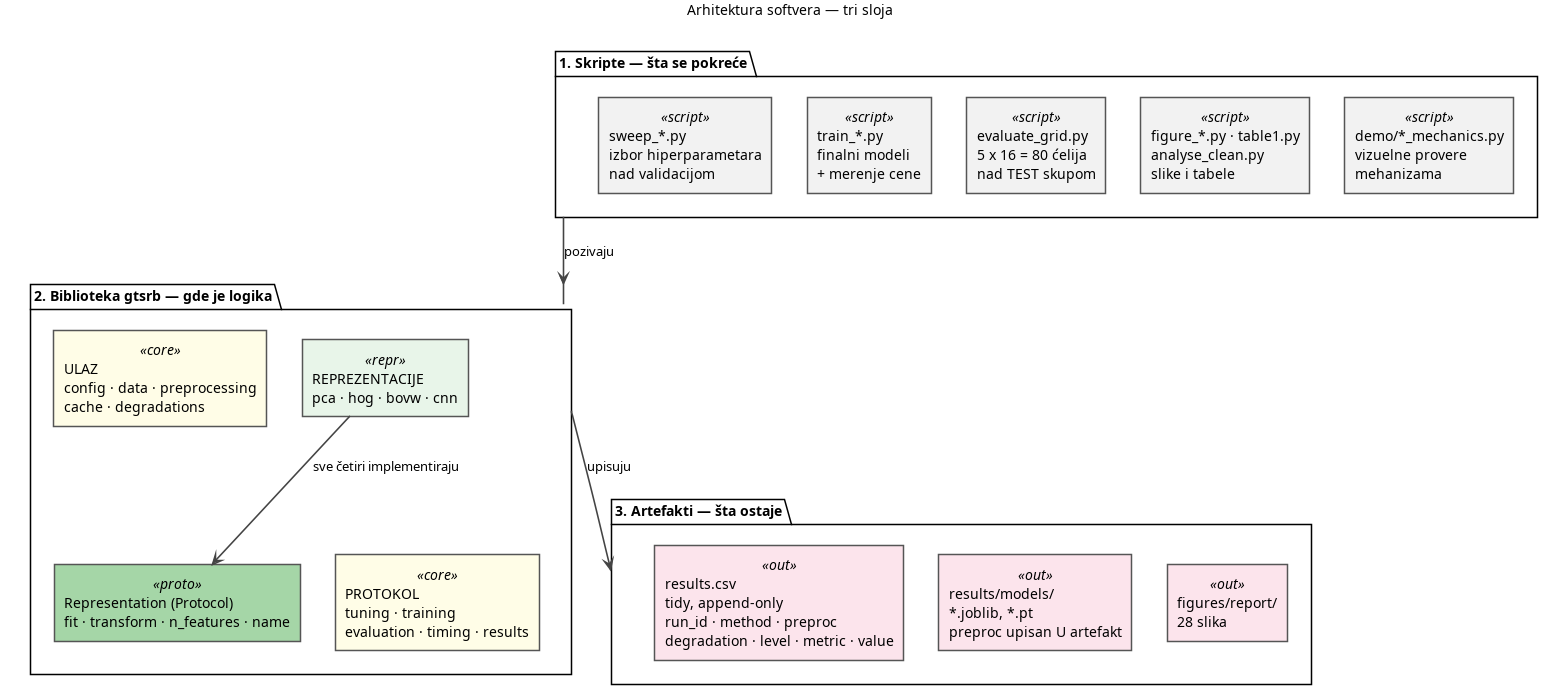
\includegraphics[width=0.82\textwidth]{architecture.png}
\end{figure}

\vspace{-0.2cm}
\small
Kod je podeljen na biblioteku \texttt{gtsrb}, gde je smeštena sva logika. 
Skripte služe za pojedinačne eksperimente, i onesamo pozivaju biblioteku i upisuju artefakte (rezultate). 
Rezultati se dopisuju u jedan \texttt{results.csv},  a uz svaki \texttt{run\_id} beleži se i okruženje u kome je merenje nastalo.

\end{frame}

\begin{frame}{Podela po sekvencama}

Slike u GTSRB skupu grupisane su u \alert{sekvence od po 30 kadrova istog fizičkog znaka}.
Nasumična podela po slikama razdvaja skoro identične kadrove na obe strane dovodeći do \textit{data leakage}-a.

\begin{figure}
\centering
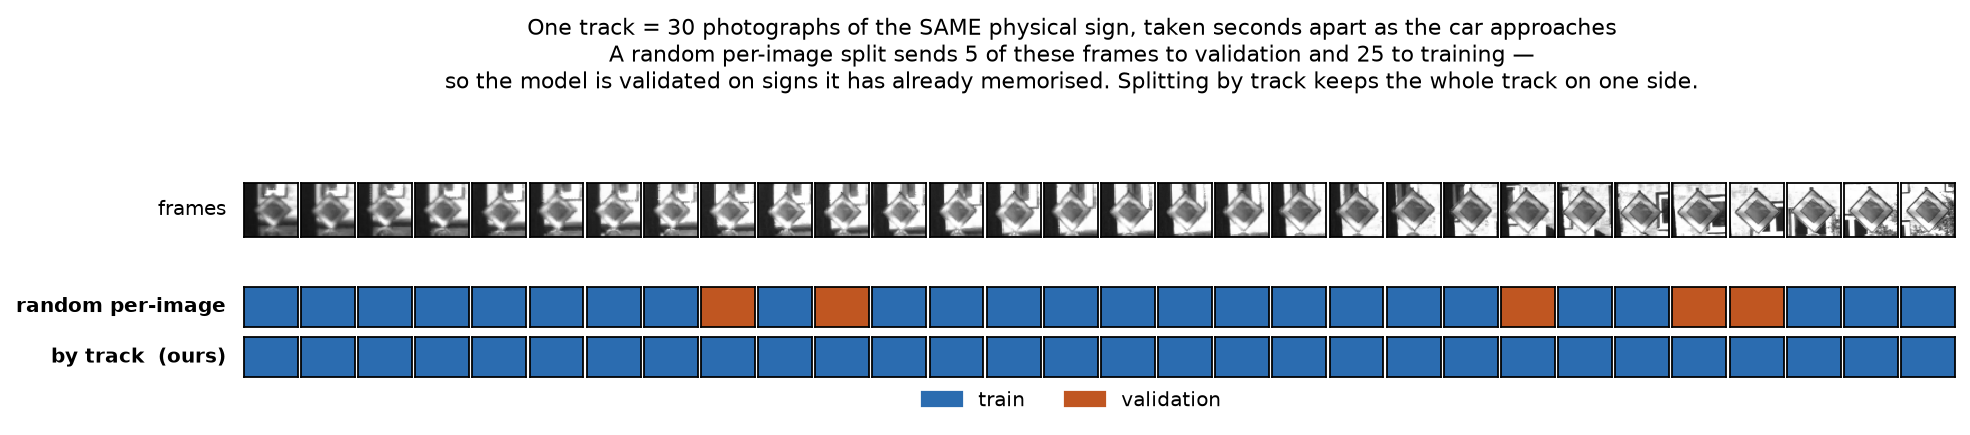
\includegraphics[width=0.86\textwidth]{split_leakage.png}
\end{figure}

\end{frame}

\begin{frame}{Mera protiv curenja podataka}

Isti model je treniran dvaput, uz jedinu razliku u pravilu podele.

\begin{center}
\begin{tabular}{lrr}
\toprule
& \textbf{podela po sekvencama} & \textbf{nasumična po slikama} \\
\midrule
validaciona tačnost  & 0,8442 & 0,8950 \quad(\alert{$+5{,}08$ pp}) \\
validacioni makro-F1 & 0,7977 & 0,8936 \quad(\alert{$+9{,}58$ pp}) \\
\bottomrule
\end{tabular}
\end{center}

\vspace{0.4cm}
\begin{block}{Zaključak koji je suptilniji i važniji}
\alert{Makro-F1 se naduvava dvostruko više od tačnosti}, jer curenje najviše pogoduje retkim
klasama. Metrika izabrana \emph{zbog} neuravnoteženosti je ona koju curenje najviše kvari.
\end{block}

\end{frame}

\begin{frame}{Tri degradacije}

Degradacije se primenjuju na \alert{pretprocesiran ulaz modela} $48\times48$, pa je ono što se
ubacuje po konstrukciji ostatak koji pretprocesiranje nije uklonilo.

\begin{figure}
\centering
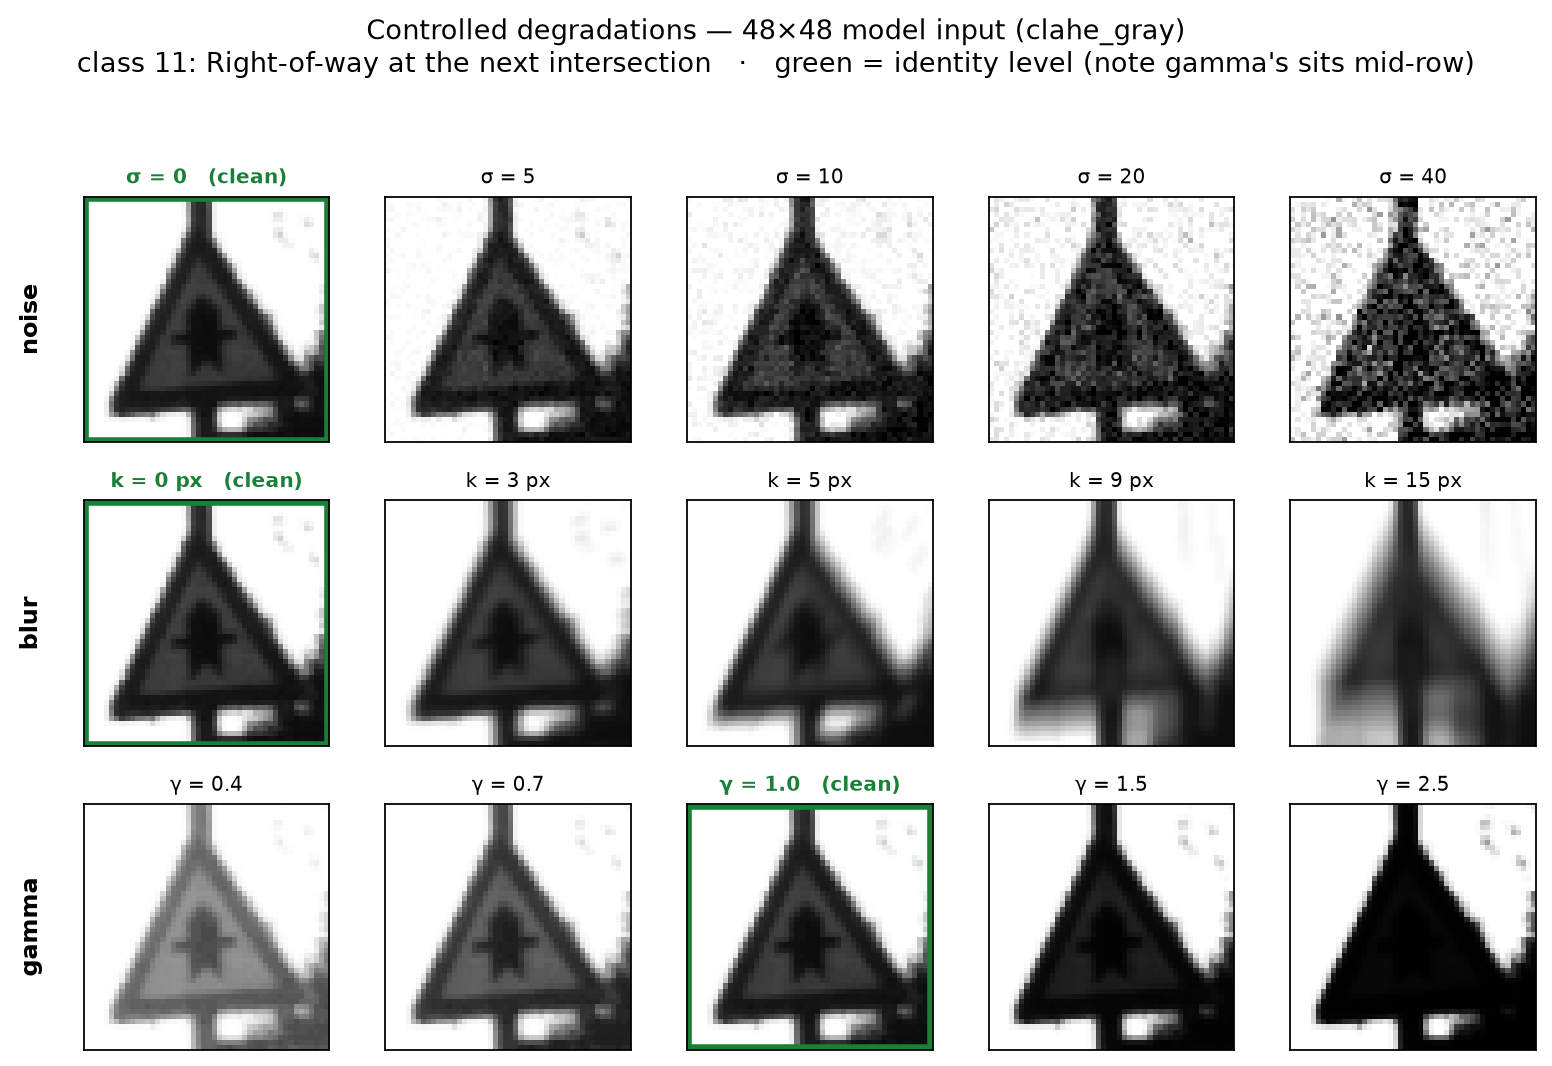
\includegraphics[width=0.54\textwidth]{degradation_contact_sheet.png}
\end{figure}

\vspace{-0.2cm}
\small
Šum \alert{dodaje} visokofrekventnu energiju, zamućenje je \alert{uklanja}, dok je gama
korekcija \alert{ortogonalna} jer geometriju ostavlja netaknutom.

\end{frame}

\begin{frame}{Očekivanja su zapisana pre prvog modela}

Napravljena unapred, pre nego što je ijedan model postojao.

\begin{itemize}
  \item \textbf{Šum} $\sigma$ 0 do 40 -- PCA najrobusnija, HOG najmanje robusna, BoVW između
        njih.
  \item \textbf{Zamućenje} $k$ 0 do 15 px -- PCA najrobusnija, BoVW najmanje robusna, uz HOG
        ispred BoVW.
  \item \textbf{Gama korekcija} $\gamma$ 0,4 do 2,5 -- HOG najrobusniji, PCA najmanje robusna.
  \item \textbf{Mali znaci} ispod 32 px -- CNN najrobusnija, BoVW najmanje robusna.
  \item \textbf{Glavno očekivanje} -- nijedna reprezentacija ne pobeđuje svuda, i
        \alert{poredak se invertuje} između vrsta degradacije. Najoštriji proverljiv slučaj
        glasi da je PCA najbolja pod šumom i najlošija pod gama korekcijom, dok za HOG važi obrnuto.
\end{itemize}

Ako se poredak pokaže stabilnim, premisa rada je pogrešna, što je svakako informativan ishod, samo zahteva drugo objašnjenje.

\end{frame}

% =====================================================================================
\section{Reprezentacije}

\begin{frame}{PCA -- holistička reprezentacija}

\begin{columns}[T]
\begin{column}{0.56\textwidth}
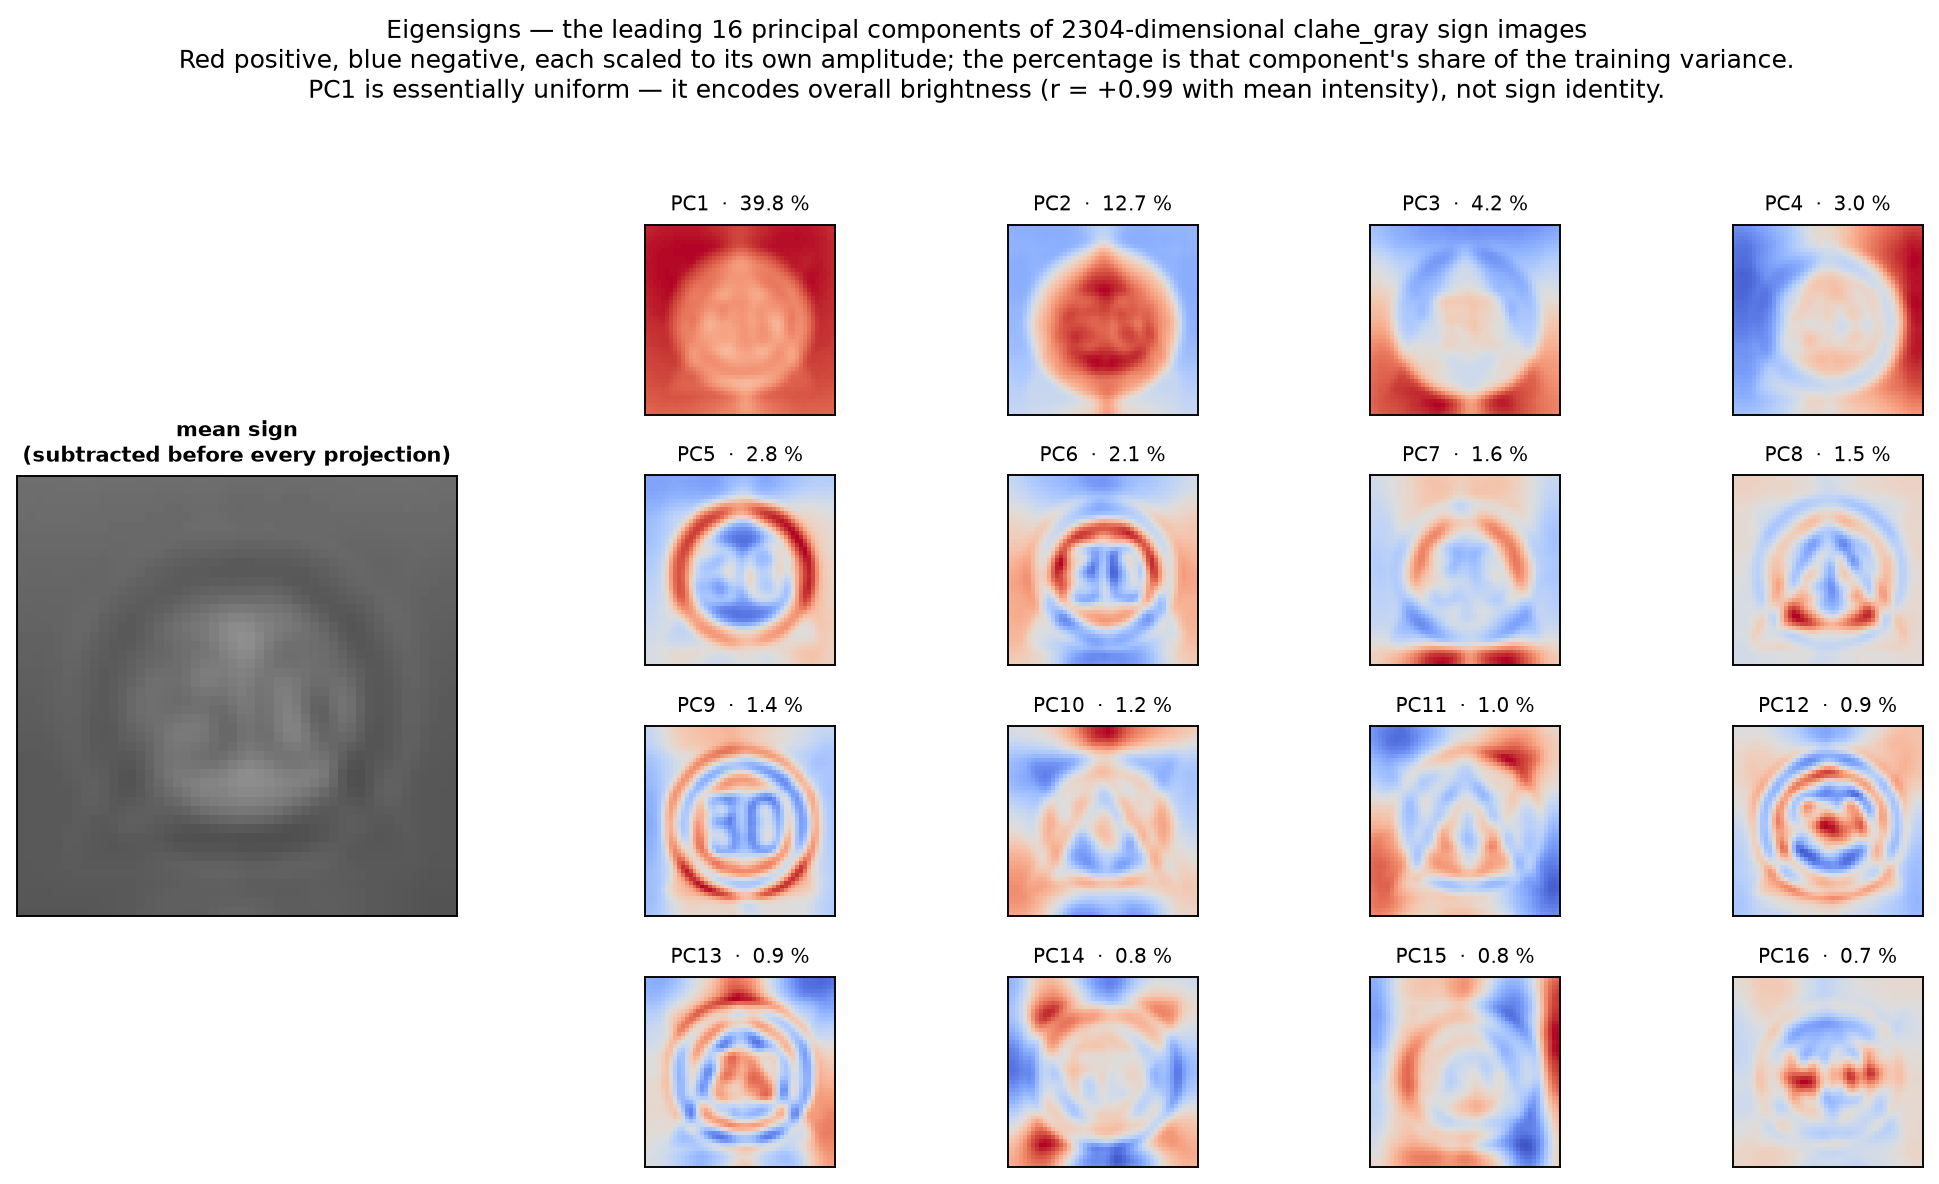
\includegraphics[width=\textwidth]{pca_eigensigns.png}
\end{column}
\begin{column}{0.42\textwidth}
\small
Prvih 16 sopstvenih vektora, uz udeo varijanse.

\vspace{0.3cm}
\textbf{PC1 je osvetljenost}, nosi $52{,}3\%$ varijanse i koreliše $+0{,}9975$ sa srednjim
intenzitetom, dakle čista smetnja.

\vspace{0.3cm}
\textbf{PC2} razlikuje okruglo od trougaonog.

\vspace{0.3cm}
Diskriminativni detalj, koja cifra i koji piktogram, predstavlja \alert{ispod $1\%$ po komponenti}.
PCA troši kapacitet po redosledu varijanse, na koji korisnost nema uticaja.
\end{column}
\end{columns}

\end{frame}

\begin{frame}{HOG -- fiksan grid, raspored očuvan}

\begin{figure}
\centering
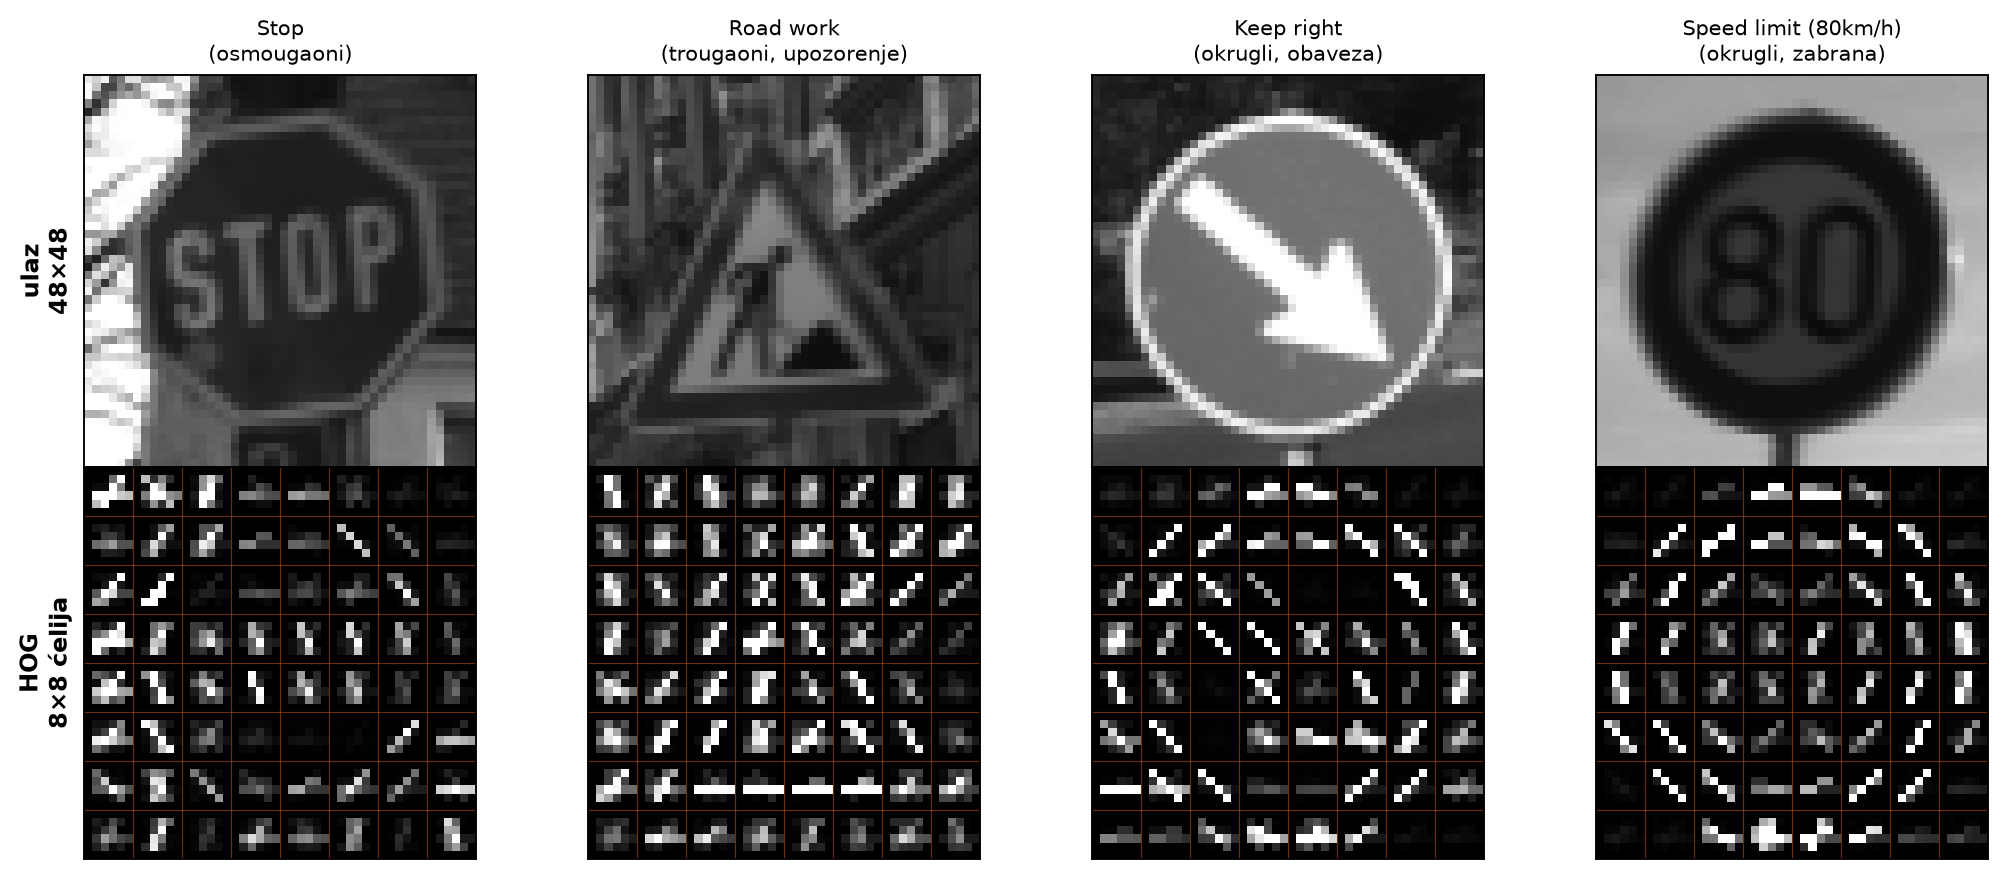
\includegraphics[width=0.84\textwidth]{hog_visualization.png}
\end{figure}

\vspace{-0.25cm}
\small
Kod znaka \textit{Speed limit (80)} kružna ivica daje snažne poteze, dok cifre daju samo
kratke i slabe. Taj detalj razdvaja 80 od 50, a gubi se pri \textit{pooling}-u unutar ćelije,
gde svi gradijenti upadaju u isti histogram od 9 orijentacija. To je najčešća greška HOG-a.

\end{frame}

\begin{frame}{BoVW -- reprezentacija bez prostornog rasporeda}

\begin{figure}
\centering
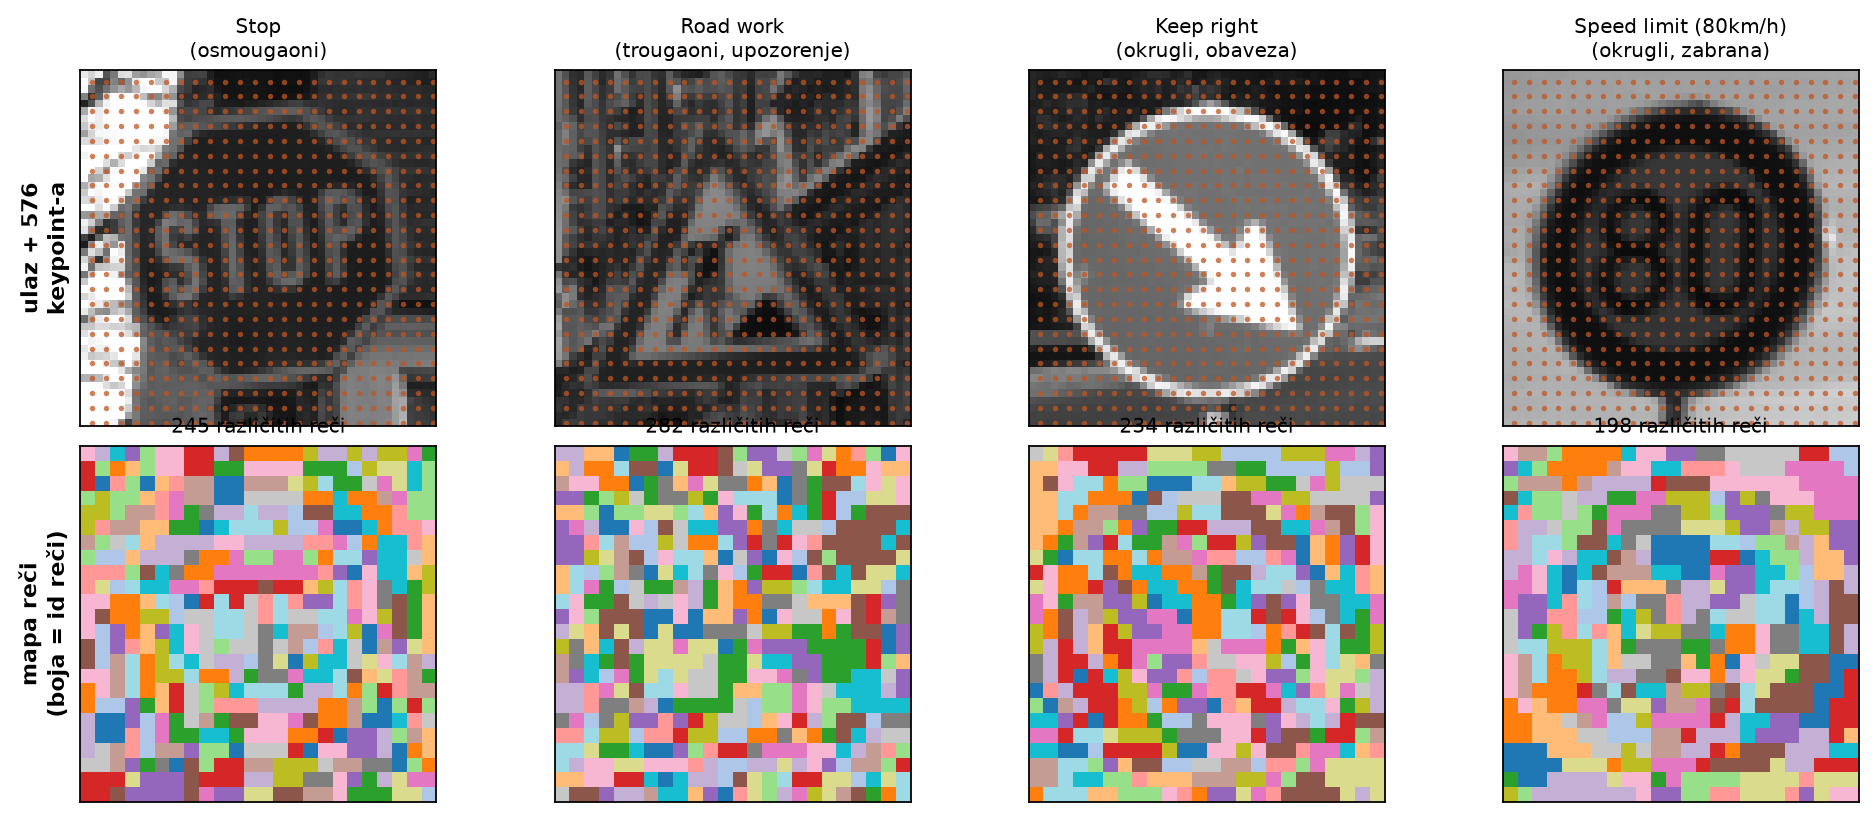
\includegraphics[width=0.80\textwidth]{bovw_grid_and_words.png}
\end{figure}

\vspace{-0.25cm}
\small
Gusti SIFT na fiksnoj mreži, pa kvantizacija na 1000 vizuelnih reči. Svaka slika doprinosi
istim brojem deskriptora, što histograme čini uporedivim. Položaj svakog \textit{patch}-a se zatim
\alert{odbacuje}.

\end{frame}

\begin{frame}{Konvoluciona mreža -- naučena reprezentacija}

\begin{columns}[T]
\begin{column}{0.60\textwidth}
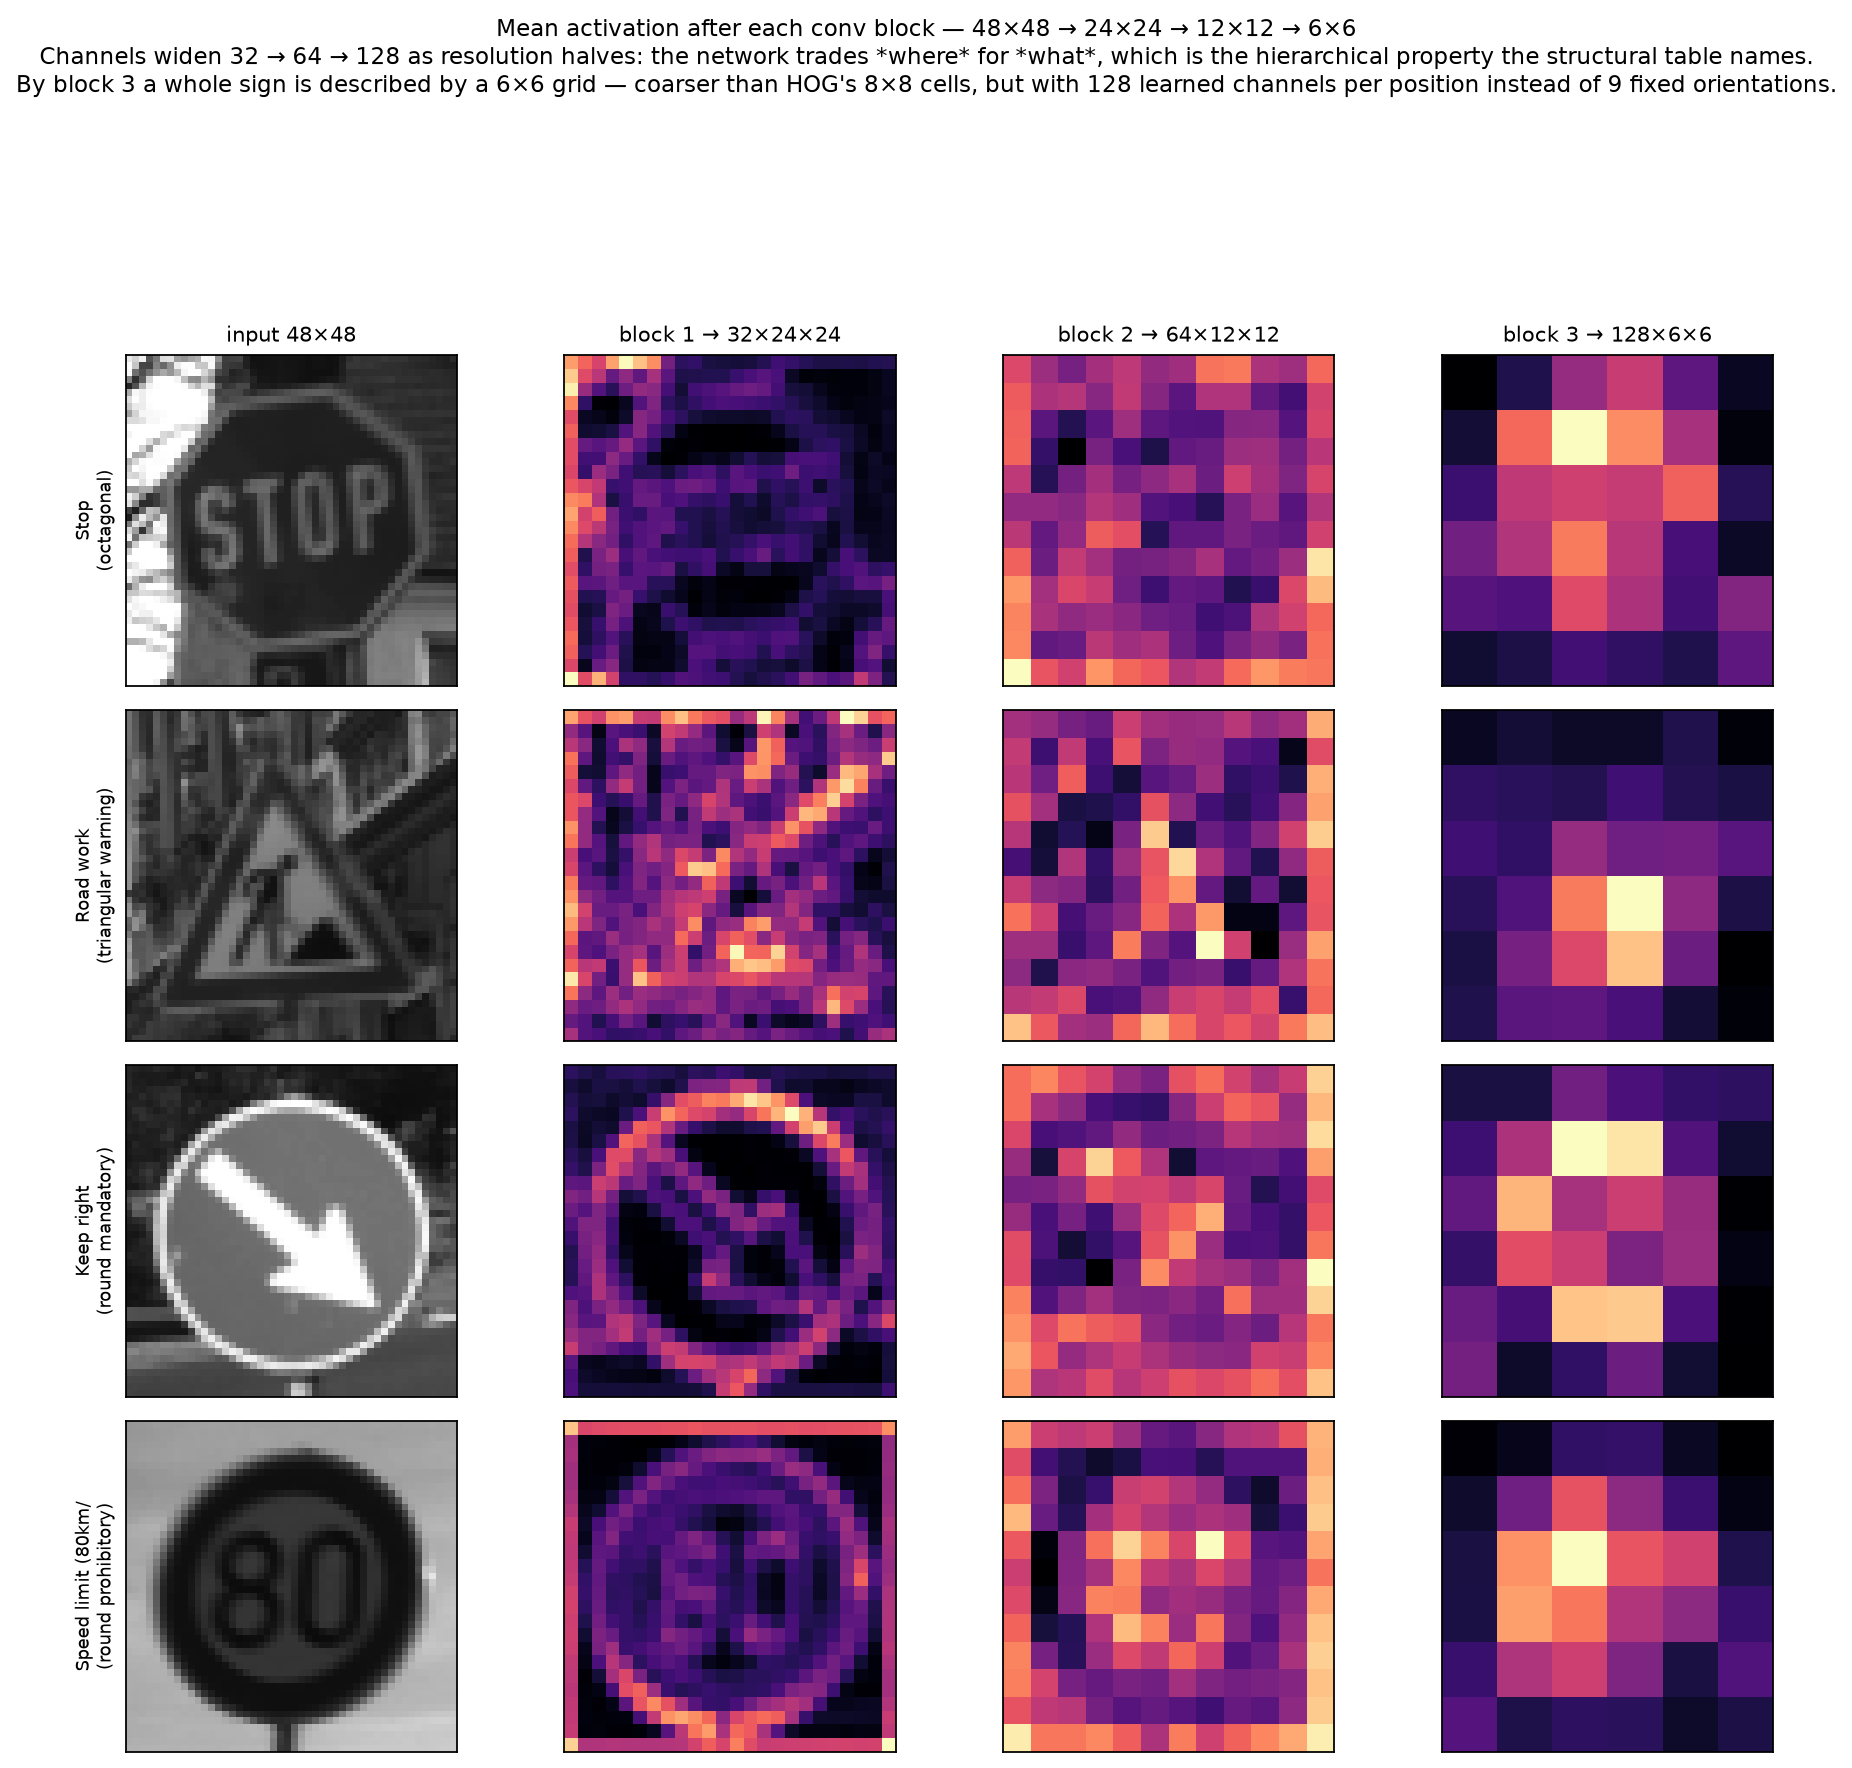
\includegraphics[height=0.70\textheight]{cnn_activations.png}
\end{column}
\begin{column}{0.38\textwidth}
\footnotesize
Rezolucija se prepolovljava $48 \to 24 \to 12 \to 6$ dok se broj kanala širi
$32 \to 64 \to 128$.

\vspace{0.3cm}
Mreža time \alert{zadržava sve manje podataka o tome \emph{gde} se nešto nalazi, a sve
više o tome \emph{šta} je}.

\vspace{0.25cm}
Do trećeg bloka znak je opisan mrežom $6\times6$, grubljom od HOG-ovih ćelija $8\times8$, ali
sa 128 naučenih kanala po poziciji.

\vspace{0.25cm}
Ukupno \alert{882.379} parametara.
\end{column}
\end{columns}

\end{frame}

% =====================================================================================
\section{Rezultati}

\begin{frame}{Rezultati na čistom test skupu}

\begin{center}
\uska
\begin{tabular}{lrrrrrr}
\toprule
\textbf{Metoda} & \textbf{Tačnost} & \textbf{makro-F1} & \textbf{Dim.} & \textbf{Trening (s)} & \textbf{1 slika (ms)} & \textbf{Model (MB)} \\
\midrule
CNN \textit{end-to-end} & 0,9785 & \alert{0,9684} & 128  & 2595,9 & 1,400 & 3,38 \\
CNN obeležja + SVM      & \alert{0,9804} & 0,9651 & 128  & 1,1$^\dagger$ & 2,037 & 0,04$^\dagger$ \\
HOG + SVM               & 0,9238 & 0,9062 & 1764 & 81,5 & 0,983 & 0,58 \\
BoVW + SVM              & 0,9141 & 0,8596 & 1000 & 89,9 & 2,792 & 1,59 \\
PCA + SVM               & 0,7932 & 0,7312 & 256  & 33,3 & 0,327 & 2,35 \\
\bottomrule
\end{tabular}
\end{center}

\vspace{0.3cm}
\small
$^\dagger$ Kolone za \texttt{cnn\_feat\_svm} nisu uporedive, jer $1{,}1$ s je vreme
\textit{fit}-ovanja samo SVM glave. Ona ne može postojati bez mreže od 2596 s koju čita, pa je
poštena vrednost $\approx 2597$ s, odnosno $3{,}42$ MB.

\vspace{0.2cm}
Na čistim podacima poredak je očekivan, uz vođstvo mreža od oko $6$ pp.

\end{frame}

\begin{frame}{Krive robusnosti -- glavni rezultat}

\begin{figure}
\centering
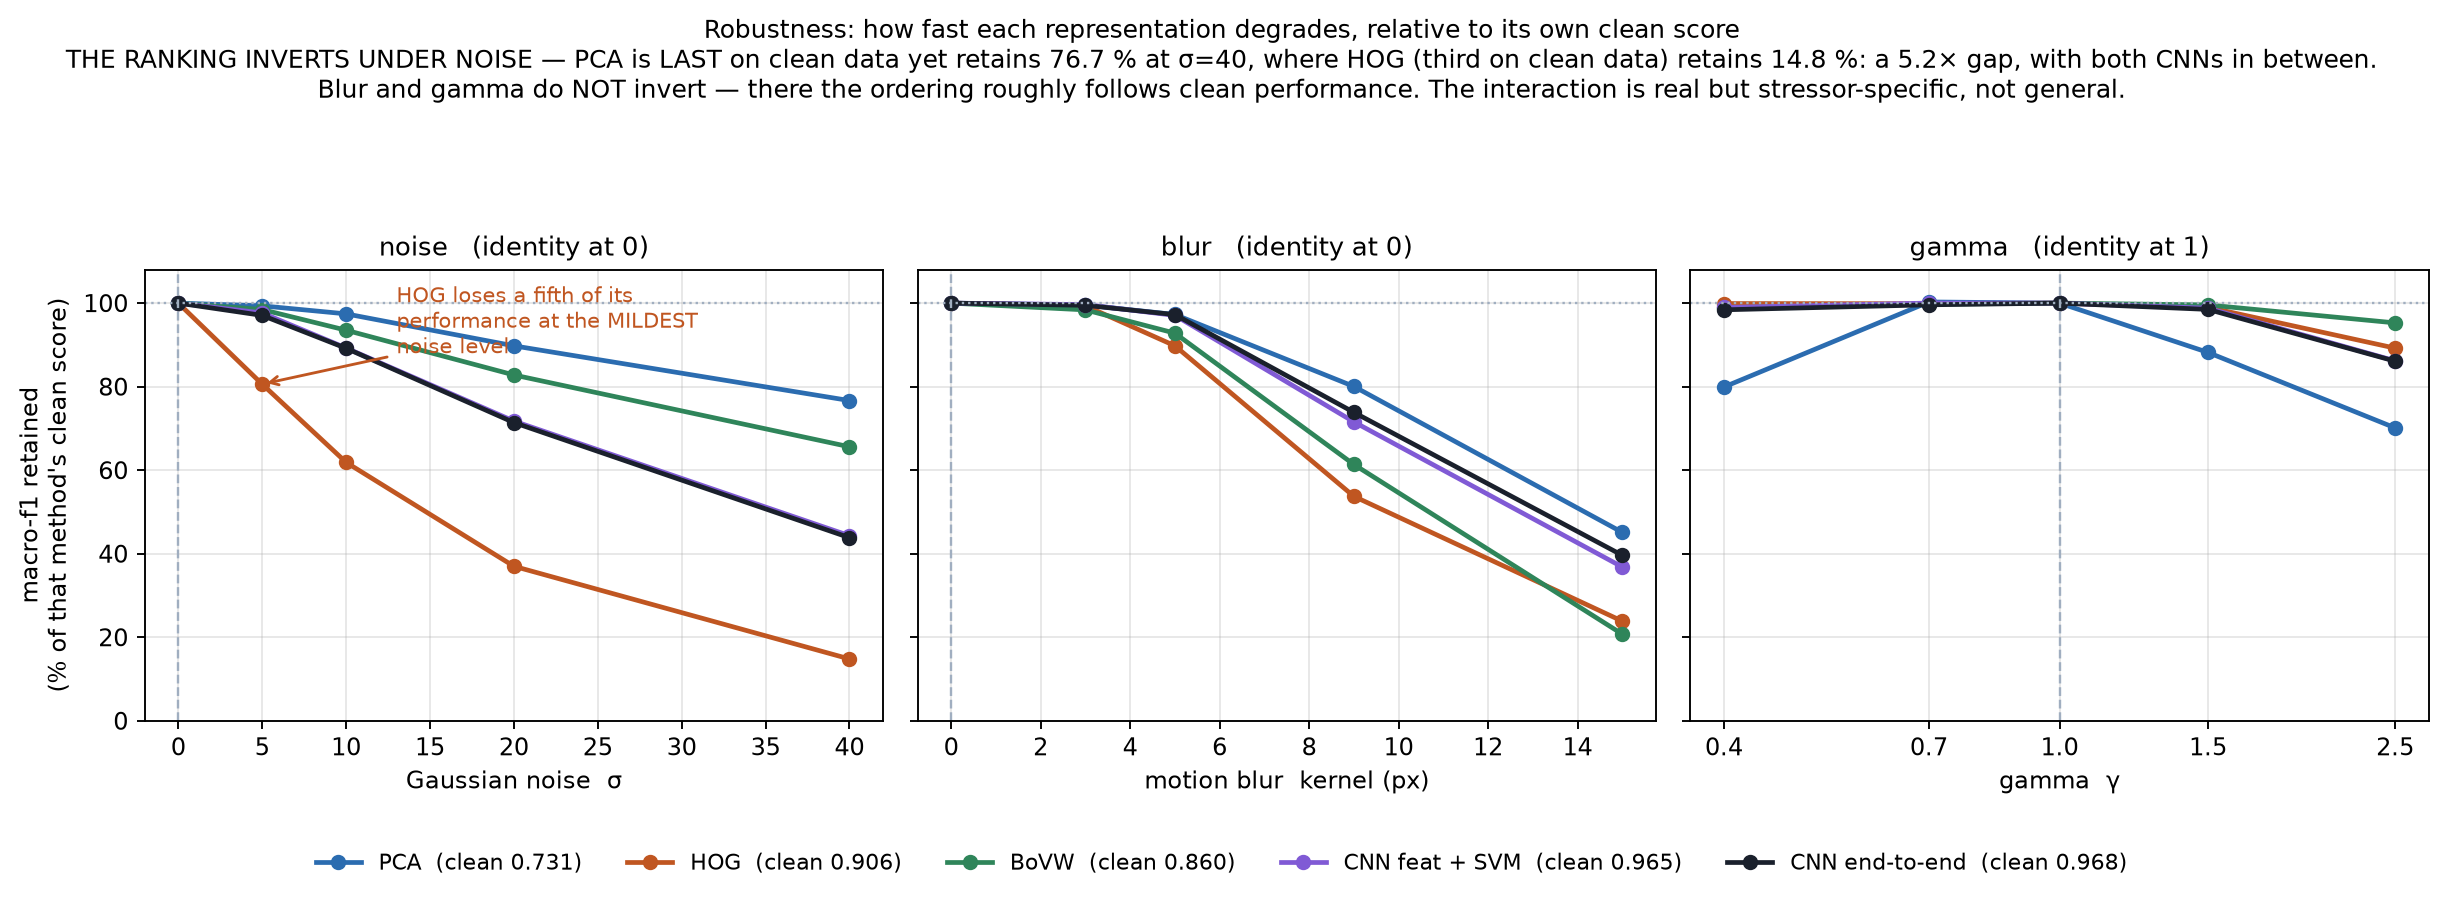
\includegraphics[width=\textwidth]{robustness_curves.png}
\end{figure}

\vspace{-0.3cm}
\small
Prikazano je zadržavanje u odnosu na sopstvenu čistu vrednost svake metode, jer je pitanje
koliko brzo svaka opada, dok o tome ko je najbolji govori prethodna tabela.

\end{frame}

\begin{frame}{Inverzija poretka pod šumom}

\begin{center}
\uska
\begin{tabular}{lrrrrr}
\toprule
\textbf{zadržano (\%)} & \textbf{PCA} & \textbf{HOG} & \textbf{BoVW} & \textbf{CNN obel.} & \textbf{CNN e2e} \\
\midrule
šum $\sigma=40$        & \alert{76,7} & \alert{14,8} & 65,6 & 44,3 & 43,8 \\
zamućenje $k=15$       & \alert{45,1} & 23,9 & \alert{20,7} & 36,8 & 39,6 \\
gama $2{,}5$           & \alert{70,1} & 89,2 & \alert{95,3} & 86,2 & 86,1 \\
\bottomrule
\end{tabular}
\end{center}

\vspace{0.35cm}
Na čistom ulazu poredak je CNN $>$ CNN-obeležja $>$ HOG $>$ BoVW $>$ PCA.
Pri $\sigma=40$ poredak postaje BoVW $>$ PCA $>$ CNN-obeležja $>$ CNN $>$ HOG, uz
Spearman-ovu korelaciju \alert{$-0{,}60$} sa čistim poretkom.

\begin{alertblock}{Napomena}
Inverzija je vezana za \emph{vrstu} degradacije. Pod zamućenjem i gama korekcijom korelacija
je $+0{,}70$ i $+0{,}90$, dakle poredak uglavnom prati čistu uspešnost. Premisa se potvrđuje,
ali je nosi jedna degradacija od tri.
\end{alertblock}

\end{frame}

\begin{frame}{Apsolutne vrednosti metrika}

\small
Zadržavanje meri brzinu opadanja, pa uz njega idu i same vrednosti. Makro-F1 na test skupu,
gde je podebljan najbolji u redu.

\begin{center}
\uska
\begin{tabular}{lrrrrr}
\toprule
\textbf{makro-F1} & \textbf{PCA} & \textbf{HOG} & \textbf{BoVW} & \textbf{CNN obel.} & \textbf{CNN e2e} \\
\midrule
čist             & 0,7312 & 0,9062 & 0,8596 & 0,9651 & \textbf{0,9684} \\
šum $\sigma=20$  & 0,6564 & 0,3352 & \textbf{0,7117} & 0,6926 & 0,6914 \\
šum $\sigma=40$  & \alert{0,5606} & 0,1341 & \alert{\textbf{0,5639}} & 0,4277 & 0,4245 \\
zamućenje $k=15$ & 0,3299 & 0,2161 & 0,1783 & 0,3554 & \textbf{0,3837} \\
gama $2{,}5$     & 0,5127 & 0,8084 & 0,8189 & 0,8318 & \textbf{0,8338} \\
\bottomrule
\end{tabular}
\end{center}

\vspace{0.15cm}
\footnotesize
\textbf{Inverzija pod šumom "preživljava" prelazak na apsolutne brojeve}, jer su pri
$\sigma=40$ PCA i BoVW izjednačeni na $0{,}33$ pp i \alert{obe nadmašuju obe mreže}. Pod
zamućenjem i gamom inverzije nema, pa tamo apsolutno vode mreže.

\end{frame}

\begin{frame}{Očekivanja naspram ishoda}

Od deset očekivanja o robusnosti, \alert{osam se obistinilo}, uključujući glavno očekivanje u
oba smera.

\begin{block}{Prvi promašaj -- presudan je \emph{tip} normalizacije}
Očekivano je da SIFT-ova zaštita od gama korekcije bude nešto slabija od HOG-ove, dok je
izmereno da je \alert{najjača u radu}. HOG-ov L2-Hys je \alert{linearan} i radi nad blokom,
dok SIFT \textit{clip}-uje svaku komponentu na $0{,}2$ pa ponovo normalizuje, što je
\alert{nelinearnost} koja potiskuje upravo komponente koje gama kriva uvećava.
\end{block}

\begin{block}{Drugi promašaj -- podešavanje je zamenilo metodu}
Očekivanje o malim znacima opisivalo je deskriptor od 12 px, koji je podešavanjem zamenjen
deskriptorom od 2 px. BoVW je ispao \alert{najstabilniji po veličini znaka}, suprotno
zapisanom.
\end{block}

\end{frame}

\begin{frame}{Cena odbacivanja prostornog rasporeda}

Prostorna piramida dodaje BoVW metodi prostorne ćelije, uz \alert{iste deskriptore, isti
rečnik i isti klasifikator}. Jedina promena je da li se položaj beleži.

\begin{center}
\begin{tabular}{lrrr}
\toprule
\textbf{Nivo} & \textbf{ćelija} & \textbf{dimenzija} & \textbf{makro-F1} \\
\midrule
0 -- obična BoVW        & 1  & 500    & 0,8143 \\
1 -- $2\times2$         & 5  & 2.500  & 0,8973 \\
\textbf{2 -- $4\times4$} & 21 & 10.500 & \alert{0,9184} \\
\bottomrule
\end{tabular}
\end{center}

\vspace{0.25cm}
Raspored vredi \alert{$+10{,}4$ pp} i dovodi metodu na $0{,}1$ pp od HOG-a. Razlika između
BoVW i HOG-a \emph{jeste} informacija o rasporedu, dok ostale razlike između te dve metode
zajedno ne daju gotovo ništa.

\vspace{0.15cm}
\small
Prikazano kao dijagnostika, jer nivo 2 pri rečniku od 1000 reči traži 21.000 dimenzija, što
je "velika cena".

\end{frame}

% =====================================================================================
\section{Zaključak}

\begin{frame}{Pet zakključaka}

\begin{enumerate}
  \item \textbf{Poredak se invertuje pod šumom}, gde PCA zadržava $76{,}7\%$ naspram
        HOG-ovih $14{,}8\%$, uz razliku od $5{,}2\times$. Inverzija je ipak vezana za vrstu
        degradacije.
  \item \textbf{Naučena obeležja nisu uvek i robusna obeležja.} Mreže vode na čistom
        ulazu za oko $6$ pp, a pod jakim šumom gube od linearne projekcije u 256 dimenzija.
  \item \textbf{Otpornost na promene intenziteta kupuje interna normalizacija}, pri čemu je
        bitan i njen tip, jer nelinearna nadmašuje linearnu.
  \item \textbf{Odbacivanje prostornog rasporeda je skupo}, specijalno kada je u pitanju dati \textit{use-case},
        izmereno na $+10{,}4$ pp.
  \item \textbf{Parametri su dominantni}, jer je podešavanje geometrije pomerilo
        BoVW za $+53{,}5$ pp i promenilo na koje je degradacije osetljiva.
\end{enumerate}

\end{frame}

\begin{frame}{Ograničenja koja rad sam navodi}

\begin{itemize}
  \item \textbf{\textit{Learning rate} mreže nikada nije podešavan}, pa je mreža jedina
        metoda čiji glavni optimizacioni hiperparametar nije biran nad validacijom. Smer je
        poznat, jer bi podešavanje moglo samo pomoći.
  \item \textbf{Treniranje je zaustavljeno pravilom \textit{early stopping}-a}, bez potvrđene
        konvergencije.
  \item \textbf{PCA sa $k=256$ i BoVW sa 1000 reči biraju vrh zadate mreže}, pa su obe
        donje granice, dok optimum nije pronađen.
  \item \textbf{Jedna konfiguracija pretprocesiranja} u finalnoj evaluaciji.
\end{itemize}

\end{frame}

\begin{frame}[standout]

Reprezentaciju treba birati prema degradaciji koja u datoj primeni dominira,
umesto prema tačnosti na čistim podacima.

\vspace{0.6cm}
\small
Za scenario u kome dominira šum pri slabom osvetljenju, PCA ili BoVW su merljivo bolji izbor
od konvolucione mreže na istom ulazu, uprkos tome što su na čistim podacima poslednji i
četvrti.

\end{frame}

% =====================================================================================
\appendix

\begin{frame}{Dodatak -- zašto \texttt{LinearSVC}}

Razvojna mašina nema upotrebljiv GPU, jer ROCm ne podržava integrisanu Vega grafiku.

\begin{itemize}
  \item Složenost kernel SVM-a je $O(n^2)$ do $O(n^3)$, pa bi nad 39.000 uzoraka trajala
        satima.
  \item Postoji i srećna okolnost za postavku, jer je linearan klasifikator \emph{slabiji},
        pa razlike između metoda ostaju razlike između reprezentacija, umesto da odraze
        koliko je klasifikator uspeo da nadoknadi.
\end{itemize}

\end{frame}

\begin{frame}{Dodatak -- protokol hiperparametara}

\begin{block}{Parametar $C$ se podešava \emph{po metodi}}
,,Fiksan klasifikator'' znači isti estimator i isti protokol izbora, dok je $C$ pomoćni
parametar. PCA je jedina reprezentacija koja nije interno normalizovana, uz raspon standardnih
devijacija obeležja od $87\times$, pa bi zamrznuta vrednost svakoj metodi dala dugme
kalibrisano za tuđu skalu.
\end{block}

\begin{block}{\texttt{class\_weight} je fiksiran na ,,balanced'' za sve}
Razlika je suštinska, jer $C$ menja jačinu regularizacije, dok \texttt{class\_weight} menja
\emph{šta je} funkcija gubitka. Vrednost ,,balanced'' odgovara makro-F1 meri, koja sve klase
tretira jednako.
\end{block}

\end{frame}

\begin{frame}{Dodatak -- šta bi \textit{whitening} uradio za PCA}

\small
\textit{Whitening} deli svaku zadržanu komponentu njenom standardnom devijacijom, pa projekcija
prestaje da bude čisto ortogonalna. Raspon standardnih devijacija obeležja pada sa
$87{,}1\times$ na $1{,}0\times$, dakle operator radi ono što tvrdi.

\begin{center}
\uska
\begin{tabular}{lrrrrr}
\toprule
\textbf{zadržano (\%)} & $\sigma=0$ & $\sigma=5$ & $\sigma=10$ & $\sigma=20$ & $\sigma=40$ \\
\midrule
bez \textit{whitening}-a & 100 & 99,3 & 97,4 & 89,8 & \alert{76,7} \\
sa \textit{whitening}-om & 100 & 98,7 & 96,7 & 88,3 & \alert{73,4} \\
\bottomrule
\end{tabular}
\end{center}

\vspace{0.1cm}
\footnotesize
Deljenje sa $\sigma$ pojačava komponente male varijanse, a to su tačno ose na kojima izotropan
šum ima najveći udeo u odnosu na signal. Mehanizam ide u predviđenom smeru, ali je
\alert{drugog reda}, jer nosi $3{,}3$ pp pri $\sigma=40$ i $-0{,}29$ pp na čistim podacima.

\begin{alertblock}{Korisnije je ono što ovo isključuje}
Whitened PCA i dalje zadržava $73{,}4\%$, naspram $\approx 44\%$ za mreže i $14{,}8\%$ za HOG.
Izvor otpornosti je \textbf{sama projekcija na potprostor}, gde 256 od 2304 dimenzije ostavlja
najveći deo energije šuma napolju. Skaliranje koordinata je samo korekcija.
\end{alertblock}

\end{frame}

\begin{frame}{Dodatak -- pretprocesiranje i defekt HSV konfiguracije}

Koliko pretprocesiranje uopšte znači prati \alert{da li reprezentacija normalizuje interno}.

\begin{center}
\uska
\begin{tabular}{lrl}
\toprule
\textbf{Metoda} & \textbf{efekat CLAHE} & \textbf{interna normalizacija} \\
\midrule
PCA  & \alert{$+2{,}64$ pp} & nema \\
HOG  & $-0{,}37$ pp & blok L2-Hys \\
BoVW & $-0{,}17$ pp & SIFT L2 + \textit{clipping} \\
CNN  & $+0{,}16$ pp & \textit{batch} normalizacija \\
\bottomrule
\end{tabular}
\end{center}

\vspace{0.3cm}
Najveći efekat pretprocesiranja ($2{,}64$ pp) manji je od najmanje razlike između metoda na
čistom test skupu ($12{,}8$ pp), čime je opravdano fiksiranje na \texttt{raw\_gray}.

\vspace{0.3cm}
\textbf{Nijansa se prelama na crvenoj}, pa su gradijenti preko te nespojivosti lažni. Cena
raste sa oslanjanjem na izvode, gde HOG gubi \alert{$9{,}70$ pp} jer bira kanal najveće
magnitude i time aktivno uzima pokvareni.

\end{frame}

\begin{frame}{Dodatak -- BoVW i $+53{,}5$ pp}

Parametri koje je plan predvideo bili su najveća greška u projektu.

\begin{itemize}
  \item \texttt{step}$=6$, \texttt{keypoint\_size}$=12$ daju makro-F1 $0{,}3455$.
  \item Podešavanje geometrije nad validacijom daje $0{,}8808$.
\end{itemize}

\begin{block}{Presudna je \emph{razmera} deskriptora, dok gustina zaostaje}
Pošto \texttt{step} fiksira broj \textit{keypoint}-a nezavisno od veličine, ta dva efekta se
razdvajaju. Pri fiksnih 256 tačaka promena razmere sa 6 na 4 px vredi $+12{,}3$ pp, dok pri
fiksnoj razmeri $2{,}25\times$ veća gustina vredi $+2{,}2$ pp.
\end{block}

Deskriptor od 12 px na isečku od 48 px opisuje četvrtinu objekta i nije lokalan ni u kom
korisnom smislu.

\end{frame}

\begin{frame}{Dodatak -- metode ne greše na istim mestima}

Broj zajedničkih parova među deset najčešćih zamena.

\begin{center}
\uska
\begin{tabular}{lrrrrr}
\toprule
& \textbf{PCA} & \textbf{HOG} & \textbf{BoVW} & \textbf{CNN obel.} & \textbf{CNN e2e} \\
\midrule
\textbf{PCA}       & 10 & 4 & 2 & \alert{0} & 1 \\
\textbf{HOG}       & 4 & 10 & 4 & \alert{0} & 1 \\
\textbf{BoVW}      & 2 & 4 & 10 & 1 & 2 \\
\textbf{CNN obel.} & 0 & 0 & 1 & 10 & \alert{6} \\
\textbf{CNN e2e}   & 1 & 1 & 2 & 6 & 10 \\
\bottomrule
\end{tabular}
\end{center}

\vspace{0.35cm}
Tri ručno projektovane metode dele greške međusobno, dok dva reda konvolucione mreže dele
šest parova međusobno i \alert{nula do dva} sa bilo čim ručno projektovanim.

\vspace{0.2cm}
Mreža nije ,,isto to, samo bolje'', već \alert{greši drugačije}, i to važi na \emph{čistim}
podacima gde svih pet metoda radi dobro.

\end{frame}

\begin{frame}{Dodatak -- cena i njena ograničenja}

\begin{itemize}
  \item \textbf{Vremena treba čitati kao indikaciju}, jer je svaka metoda merena tokom
        sopstvenog izvršavanja, pri različitom opterećenju sistema. Prenos na drugu platformu
        može promeniti poredak, a mreža je sistematski kažnjena odsustvom GPU-a.
  \item \textbf{Veličina modela nije uporediva ni između ostalih redova.} Kod PCA je $96\%$ od
        $2{,}35$ MB naučena baza, dok HOG nema nijednu \textit{fit}-ovanu fazu, pa je njegovih
        $0{,}58$ MB u celosti SVM.
  \item \textbf{Odnos \textit{batch} i pojedinačne inferencije je specifičan za metodu}, uz
        raspon od PCA $52\times$ do CNN $1{,}4\times$. Kamera daje jedan kadar u jednom
        trenutku, pa je pojedinačna kolona ona koju sme koristiti bilo kakva tvrdnja o
        kašnjenju, i u njoj se prednost PCA metode svodi sa $200\times$ na $8{,}5\times$.
\end{itemize}

\end{frame}

\end{document}
